\section{Simulations}

\newcommand*{\Scale}[2][4]{\scalebox{#1}{$#2$}}%

Using Duhamel's priciple, the analytic solution to Fick's second law on a half-infite line is
\[\Scale[0.5]{\phi (x,t) = KC_{out} - \int \limits_0^t erf(\frac{x}{\sqrt{4D(t - \tau)}})K\dot{C_{out}}(\tau)d\tau - KC_{out}(0)erf(\frac{x}{\sqrt{4Dt}}),}\]
where $K$ is the solubility of the material, $D$ is the diffusion constant, and $C_{out}$ is the outside concentration of the material. \cite{Piche} For the out gassing process we are only able to detect the flux of material out of the plastic.  This is given by Fick's first law evaluated at $x=0$,
\[J_{out}(t)= - K \sqrt{\frac{D}{\pi}}( \int \limits_0^t \frac{\dot{C_{out}}(\tau)}{\sqrt{t-\tau}} d \tau + \frac{C_{out}(t)}{\sqrt{t}}),\]
where the sign has been flipped since the flux of material is outward.  We see that it is no longer possible to evaluate $K$ and $D$ separately, since the diffusion in and out of the plastic is completely determined by the time-dependent concentration outside of the plastic.  To simplify our model, we define a new constant
\[ G = K \sqrt{ \frac{D}{ \pi }} .\]

We can fit the integral of our equation for the flux out of the plastic over time to out gassing data collected in Maryland's liquid xenon system to extract a value for the constant $G$.  With this method we constrain $G \leq 0.01 \; \frac{cm}{\sqrt{day}}.$ 


\subsection{Implications for LUX}

With a constraint on $G$ taken from the analytic solution to Fick's second law, we turn to numerical simulation to answer the question of how much initial CH$_3$T activity to inject into LUX to meet our calibration conditions.  Several assumptions are made to simplify the numerical model.  First, we approximate the diffusion into plastic as being a one dimensional process.  Since the plastic in our detector at Maryland and in LUX can be approximated by a cylindrical shell, there is no dependence on the azimuthal or $z$ coordinates.  Since $r$ is large compared to the thickness of the plastic shell, $\frac{\delta^2 \phi}{\delta r^2} \gg \frac{1}{r} \frac {\delta \phi}{\delta r}$, so Fick's laws in a one dimensional approximation become
\[J=-D\frac{\delta \phi}{\delta r}\vec{r}\]
\[\frac{\delta \phi}{\delta t} = D \frac{\delta^2 \phi}{\delta r^2}.\]  We assume the concentration of CH$_3$T in LUX is uniform throughout its volume, since the design of LUX creates currents which stir the liquid xenon.  With perfect mixing the effect of the purifier can be modeled by adding an exponential time dependence to the outer volume.  The time constant of this decay has an upper limit equal to the time it takes xenon to recirculate through the LUX detector, although in reality the mass transport from diffusion in the liquid and gaseous xenon decreases this time constant. 

We use a simple implementation of the first order Euler method for our numerical simulations. The diffusion is simulated by setting the concentration at the boundary of the piece equal to $KC_{out}$, where $C_{out}$ is the concentration of CH$_3$T in the xenon.  This concentration is dependent on time according to
\[\frac{\delta C_{out}}{\delta t} = J_{out} \frac{A_{plastic}}{V_{xenon}}-\frac{C_{out}}{\tau},\]
where $A_{plastic}$ is the surface area of the plastic cylinder, $V_{xenon}$ is the total volume of xenon in the fiducial region, and $\tau$ is the time it takes for one full purification cycle.  The first term on the right of this equation models out gassing of CH$_3$T from the plastic cylinder, while the second term models removal of CH$_3$T through purification.  Using the first order Euler method, we arrive at an expression for $C_{out}$ given by
\[C_{j+1}=C_j + \Delta t [(J_{1,j}-J_{N_x,j})\frac{A_{plastic}}{V_{xenon}}-\frac{C_j}{\tau}].\]
The initial concentration is defined by dividing the desired injection activity by the volume of the fiducial region.  We choose $D = 2.3 \times 10^{-9} \frac {cm^2}{sec}$ so that the half-infinite boundary conditions in our diffusion model is valid, and combine this with our allowed range of values for $G$ to extract a value for $K$.  We use this model to predict the total number of calibration events as well as the time required to return to \textless 5\% of the nominal background rate for any CH$_3$T injection into LUX.  

\begin{figure}[h]
\centering
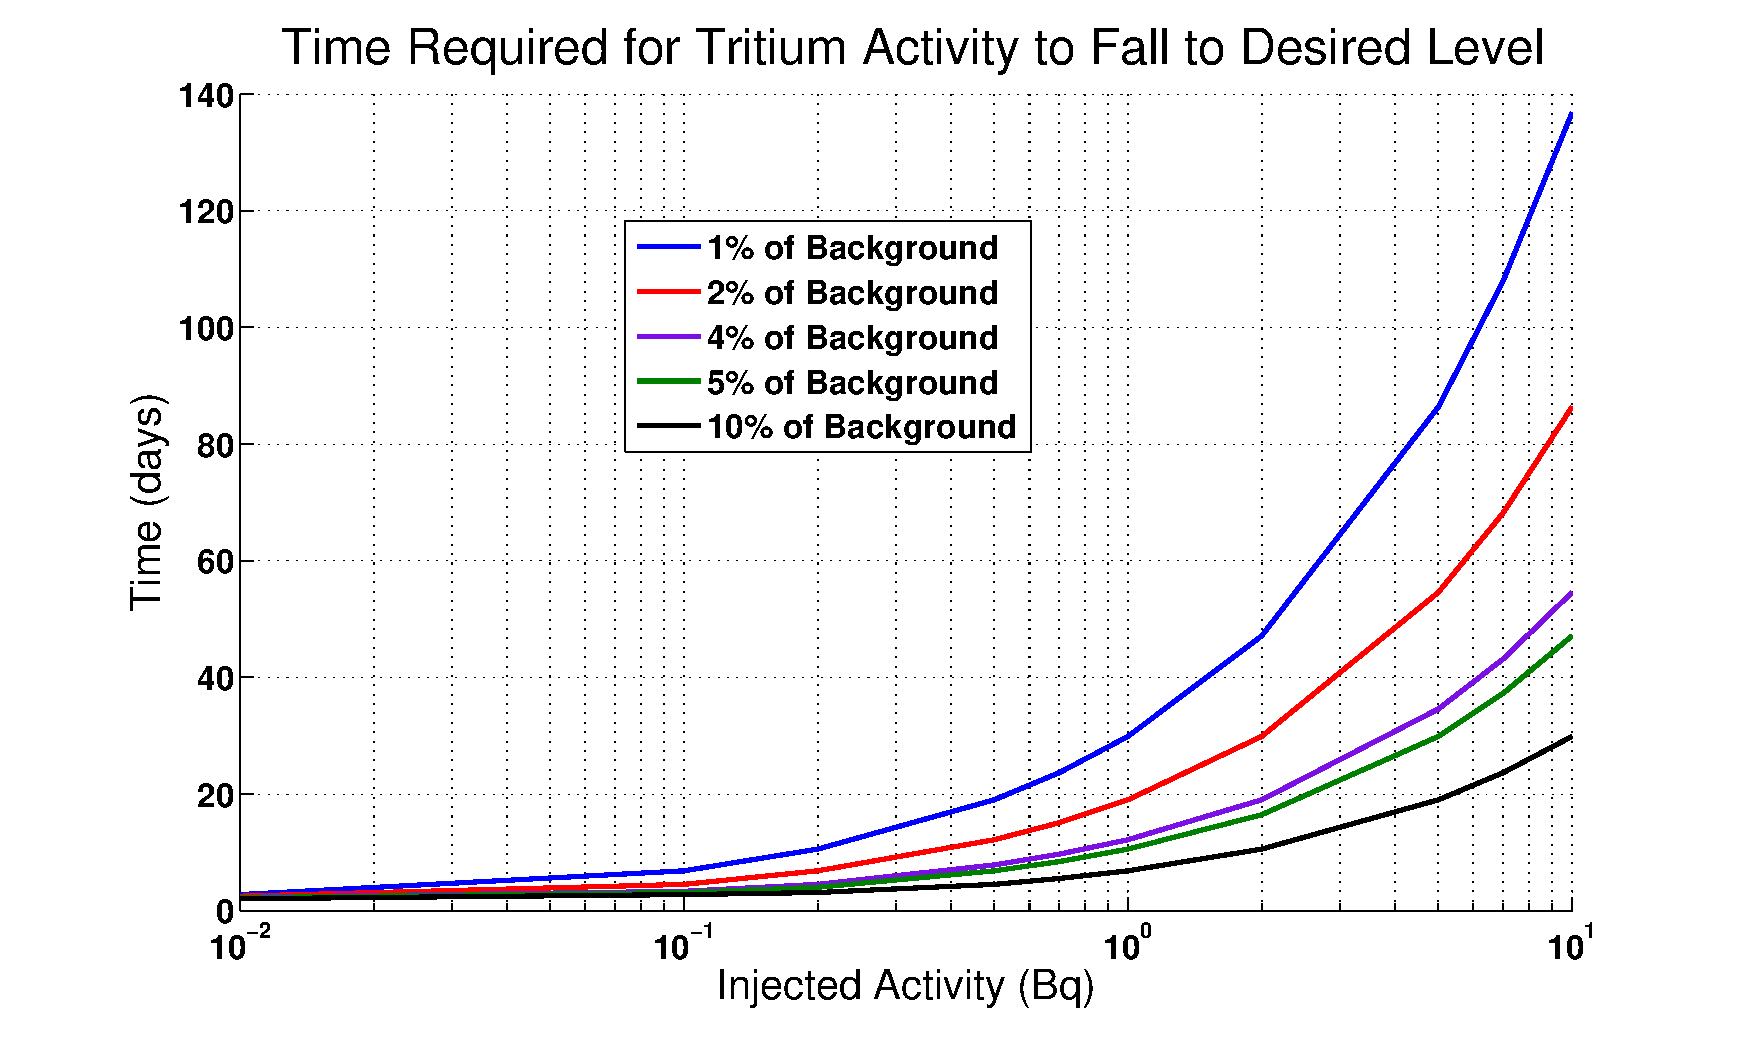
\includegraphics[scale=0.25]{LUXfig_INJvar_time_new.eps}
\caption{Time required to remove CH$_3$T from LUX after various injections.}
\label{fig:CH3TREMOVAL}
\end{figure}